%% V0.1
%% by Luis Batista, luisfelipew@gmail.com
%% This is a template for Udacity projects using IEEEtran.cls


\documentclass[10pt,journal,compsoc]{IEEEtran}

\usepackage[pdftex]{graphicx}    
\usepackage{cite}
\usepackage[table,xcdraw]{xcolor}
\usepackage{amssymb}
\usepackage{float}
\usepackage{caption}
\usepackage{subcaption}


\hyphenation{op-tical net-works semi-conduc-tor}
\graphicspath{{img/}}


\begin{document}

\title{Project: Where Am I?}

\author{Luis F. W. Batista}

\markboth{Localization project, Robotics Nanodegree Program, Udacity}%
{}
\IEEEtitleabstractindextext{%

\begin{abstract}
This report presents a theoretical comparison between Extended Kalman Filters and Adaptative Monte Carlo localization, two widely-used algorithms for localization in robotics.
For evaluation, two robot models, are implemented in a ROS package. Using AMCL and Navigation packages, the robots transverses through a simulated map with obstacles and reach a specified position. An outline of the components used is explained along with an overview of how the parameters were adjusted to enable the robots to successfully reach the target.
\end{abstract}

\begin{IEEEkeywords}
Robot, IEEEtran, Udacity, \LaTeX, Localization, ROS, Gazebo, Kalman Filter, AMCL.
\end{IEEEkeywords}}


\maketitle
\IEEEdisplaynontitleabstractindextext
\IEEEpeerreviewmaketitle
\section{Introduction}
\label{sec:introduction}

\IEEEPARstart{A}{utonomous} robots must be able to navigate through space based on information provided by sensors. In order to plan the path and control the actuators, the robot must be able to estimate its position on a given map. This task is known as Localization and is fundamental competence required by a robot. Knowing its own location is an essential precursor to deciding future actions \cite{localization}. 

Several approaches exist to solve the localization problem. 
Two popular localization algorithms are Extended Kalman Filter Localization Algorithm (EKF) \cite{ekf} and the Adaptive Monte Carlo Localization Algorithm (AMCL) \cite{thrunpr}.

The main goal of this project is to experiment with the localization algorithms. In order to achieve that, AMCL and Navigation Stack packages form ROS are used to localize and move the robot in a simulated environment using Gazebo.

Two robot models are used for evaluation. The box-shaped Udacity Bot and the R2D2 Bot, loosely resembling the iconic robot from Star Wars. By observing the results in RViz, the parameters of each algorithm are tuned to enable the robots to navigate through the map and reach a given position.



\section{Background}

Localization is fundamental for developing autonomous mobile robots. In order to decide where to move, the robot first needs to estimate its position. In the real world, sensors are noisy and actuators might not be very precise. Moreover, external influences such as wind, slippage and many others. This combination increases the challenges of implementing a precise localization.

The localization problem can be separated into three different types: local localization, global localization, and kidnapped robot. The local localization is the simplest, where the robot's pose is known and it is necessary to update its position as it moves despite the sensors noise. The global localization is when the initial pose of the robot is unknown. The last problem is known as the kidnapped robot, where at any given time the robot can be moved to another location in the map.

In this paper, Kalman Filters and the Monte Carlo Localization algorithms are compared, and the Adaptative Monte Carlo Localization algorithm is evaluated in a simulated environment.




\subsection{Kalman Filters}
The Kalman Filter (KF) is one of the most practical algorithms to estimate the state of a system based on uncertain information such as noisy sensors. It was first introduced by Rudolf E. Kálmán and used in trajectory estimation for the Apollo program. It can achieve accurate results without a lot of data and does not require many computational resources.

Kalman filters have a probabilistic approach to improve the accuracy of the estimations and can be used to solve local localization problems. First, an initial prediction of the state is made. Next, starts a cycle of state prediction and measurement update. This cycle is continuously repeated using sensor data provided in real time.

Traditional Kalman Filters assume that the system is linear. However, it is not the case in many applications. One solution is to approximate a non-linear equation using some terms from the Taylor Series. This is known as Extend Kalman Filters and they are widely used in the field of Robotics.


\subsection{Particle Filters}
Particle filters are another common approach to solve to Localization problem in Robotics. The particles are virtual elements that represent possible positions and orientations of the robot. The algorithms can estimate the actual pose of the robot by randomly distributing the particles across the map and filtering the ones that are more likely to be correct by comparing with sensor information. 

Opposed to the EKF, the MCL algorithm can be successfully used in Global Localization problems. Moreover, the measurement noise is not restricted to Gaussian distribution which makes it a good option in several applications.

The computational power required proportional to the number of particles used. The Adaptative Monte Carlo Localization algorithm adjusts the number of particles according to the overall accuracy of the estimation, making it possible to lower the computational resources required and the particle distribution converges.


\subsection{Comparison / Contrast}
Given their intrinsic characteristics, each algorithm can be more suitable for different applications. The Table \ref{tab:algo-comparison} presents a summary of the key differences between each other. 

\begin{table}[H]
\centering
\begin{tabular}{|l|c|c|}
\hline
\rowcolor[HTML]{C0C0C0} 
\multicolumn{1}{|c|}{\cellcolor[HTML]{C0C0C0}\textbf{amcl parameter}}   & \textbf{Udacity Bot}                                          & \textbf{R2D2 Bot}   \\ \hline
Measurements           & Raw Measurements     & Landmarks             \\ \hline
Measurement Noise      & Any                  & Gaussian              \\ \hline
Posterior              & Particles            & Gaussian              \\ \hline
Efficiency (memory)     & \checkmark           & \checkmark\checkmark  \\ \hline
Efficiency (time)      & \checkmark           & \checkmark\checkmark  \\ \hline
Ease of implementation & \checkmark\checkmark & \checkmark            \\ \hline
Resolution             & \checkmark           & \checkmark\checkmark  \\ \hline
Robustness             & \checkmark\checkmark & X                     \\ \hline
\begin{tabular}[c]{@{}l@{}}Memory and\\ Resolution Control\end{tabular} & yes  & no \\ \hline
Global Localization    & yes                  & no                    \\ \hline
State Space     & \begin{tabular}[c]{@{}c@{}}Multimodal\\ Discrete\end{tabular} & \begin{tabular}[c]{@{}c@{}}Unimodal\\ Continuous \end{tabular} \\ \hline
\end{tabular}
\caption{MCL and EKF Comparison}
\label{tab:algo-comparison}
\end{table}

Kalman Filter would be a good choice to be used in a system with high computational restrictions and where the measurement noise has a Gaussian distribution. If solving global localization is important. MCL is a better alternative. While it requires higher computational resources, it can be controlled by adjusting the number of particles. 

The work presented in this report will focus only on the particle filter approach. More specifically using the AMCL implementation available in ROS.


\section{Simulations}

The Gazebo simulation environment was used to test and experiment with the AMCL algorithm. Two robot models were used for comparison. 
 
Using the AMCL and Navigation packages and the ROS environment, the robots had to navigate through the provided map shown in Figure \ref{fig:jackal-map}, and reach a given position. The performance was compared by observing the convergence of the particles displayed in RViz and the time needed to reach the final pose. 

\begin{figure}[H]
  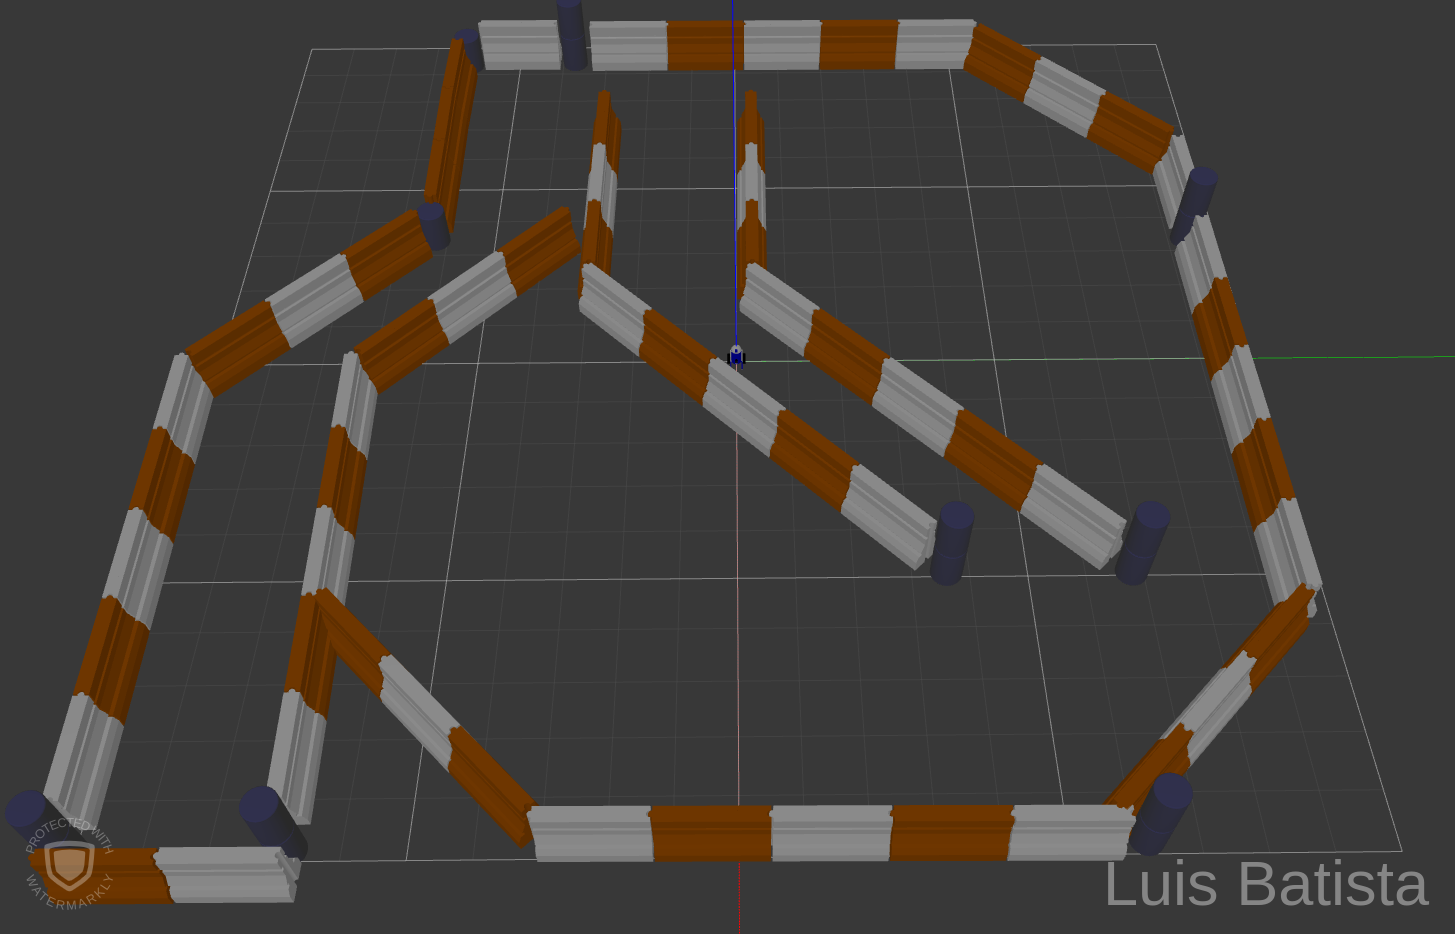
\includegraphics[width=\linewidth]{jackal_map.png}
  \caption{Jackal Race Map}
  \label{fig:jackal-map}
\end{figure}

\subsection{Achievements}

After adjusting the parameters, the calculated particles converged and allowed the robots to navigate through the map. Both models were able to successfully reach the goal position in less than 65 seconds.

\subsection{Model design}
\label{sec-modeldesign}
The simulation was done with two different models. A benchmark model, referred as Udacity Bot (Figure \ref{fig:ub-model}), and a personal model, referred as R2D2 Bot (Figure \ref{fig:r2d2-model}). The benchmark model was provided by Udacity along with the course materials. The R2D2 Bot kept the same wheels but its chassis was redesigned to resemble the R2D2 robot from the Star Wars movie.


\begin{figure}[H]
\centering
\begin{subfigure}{.5\linewidth}
  \centering
  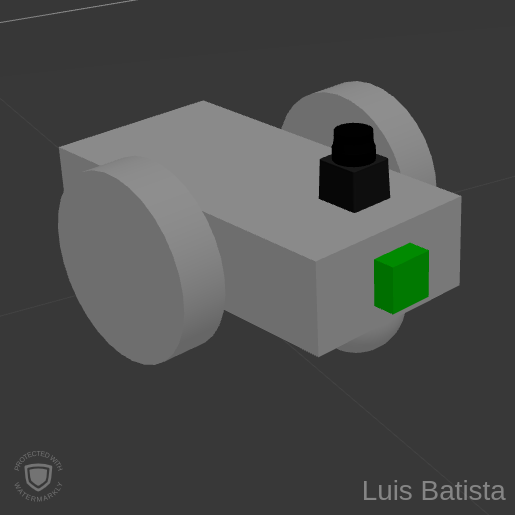
\includegraphics[width=.95\linewidth]{ub_model2.png}
  \caption{Udacity Bot}
  \label{fig:ub-model}
\end{subfigure}%
\begin{subfigure}{.5\linewidth}
  \centering
  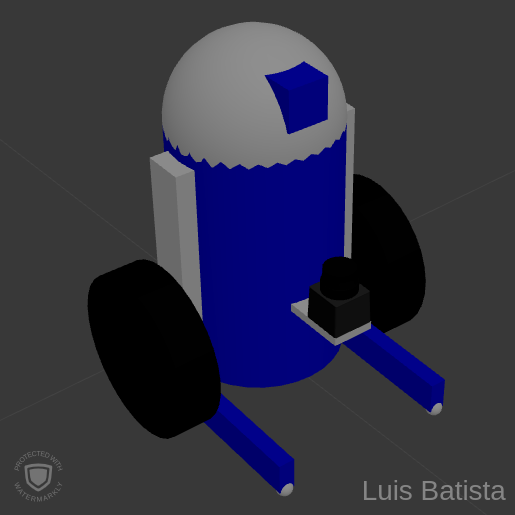
\includegraphics[width=.95\linewidth]{r2d2_model2.png}
  \caption{R2D2 Bot}
  \label{fig:r2d2-model}
\end{subfigure}
\caption{Robot Models}
\label{fig:models}
\end{figure}


The mass, inertia, footprint, and wheel design were kept as similar as possible to minimize the variables that could impact on simulation results. The goal was to enable a better comparison of the AMCL and navigation parameters. For detailed information about the robot models, please refer to the implementation code available \cite{luisfelipewb-repo}.

Both robots have a camera and a laser sensor. The camera is not used for localization and in the R2D2 Bot, it was repositioned in the head of the robot. The location of the Laser sensor was kept in the same position to guarantee similar measurements results. If the hight was changed, it would be expected that the measured distance would vary given that the base of the obstacles has an angled surface.

\subsection{Packages Used}
The robot models were implemented in a ROS package called \textit{udaicty-bot}. In order to spawn the correct robot model, it is only necessary to adjust which robot description is included in the \textit{world.lauch} file.

To implement localization and movement of the robots, the following packages were used:
\begin{itemize}
	\item \textbf{amcl} - Package used for localization. By adjusting a set of parameters it is possible to customize the overall behavior of the filter. It can also be adjusted based on the laser and odometry specifications.
	\item \textbf{move base} - Package used to calculate the path and control the robot to reach the goal.
	\item \textbf{xacro} - Package used to describe the robot model. It parses a simplified description and generates the full urdf XML description of the robot.
\end{itemize}


\subsection{Parameters}

For comparing the localization performance, different parameters were used for each robot. 
The Table \ref{tab:amcl-param} shows the final parameters of the amcl package and the parameters used in the move base package are listed in Table \ref{tab:blc-param}. Note also that the costmap parameters, described in Table \ref{tab:costmap-param}, remained unchanged in final tests. 


\begin{table}[H]
\centering
\begin{tabular}{|l|c|c|}
\hline
\rowcolor[HTML]{C0C0C0} 
\multicolumn{1}{|c|}{\cellcolor[HTML]{C0C0C0}\textbf{amcl parameter}} & \textbf{Udacity Bot} & \textbf{R2D2 Bot} \\ \hline
min\_particles         & 10                   & 20                \\ \hline
max\_particles         & 100                  & 500               \\ \hline
update\_min\_d         & 0.05                 & 0.001             \\ \hline
update\_min\_a         & \( \pi \)/6          & 0.001             \\ \hline
resample\_interval     & 2                    & 1                 \\ \hline
trasnform\_tolerance   & \multicolumn{2}{c|}{0.1}                 \\ \hline
laser\_min\_range      & \multicolumn{2}{c|}{0.1}                 \\ \hline
laser\_max\_range      & \multicolumn{2}{c|}{10.0}                \\ \hline
laser\_model\_type     & \multicolumn{2}{c|}{likelihood\_field}   \\ \hline
odom\_model\_type      & \multicolumn{2}{c|}{diff-corrected}      \\ \hline
base\_frame\_id        & \multicolumn{2}{c|}{robot\_footprint}    \\ \hline
\end{tabular}
\caption{amcl parameters}
\label{tab:amcl-param}
\end{table}

\begin{table}[H]
\centering
\begin{tabular}{|l|c|c|}
\hline
\rowcolor[HTML]{C0C0C0} 
\multicolumn{1}{|c|}{\cellcolor[HTML]{C0C0C0}\textbf{base\_local\_planner parameters}} & \textbf{Udacity Bot} & \textbf{R2D2 Bot} \\ \hline
controller\_frequency   & \multicolumn{2}{c|}{10}                  \\ \hline
holonomic\_robot        & \multicolumn{2}{c|}{false}               \\ \hline
yaw\_goal\_tolerance    & 0.05                 & 0.1               \\ \hline
xy\_goal\_tolerance     & \multicolumn{2}{c|}{0.1}                 \\ \hline
meter\_scoring          & \multicolumn{2}{c|}{true}                \\ \hline
\end{tabular}
\caption{base\_local\_planner parameters}
\label{tab:blc-param}
\end{table}

\begin{table}[H]
\centering
\begin{tabular}{|l|c|c|}
\hline
\rowcolor[HTML]{C0C0C0} 
\multicolumn{1}{|c|}{\cellcolor[HTML]{C0C0C0}\textbf{Udacity and R2D2}} & \textbf{global\_costmap} & \textbf{local\_costmap} \\ \hline
map\_type            & \multicolumn{2}{c|}{costmap}                                                                 \\ \hline
obstacle\_range      & \multicolumn{2}{c|}{3.0}                                                                     \\ \hline
raytrace\_range      & \multicolumn{2}{c|}{8.0}                                                                     \\ \hline
transform\_tolerance & \multicolumn{2}{c|}{0.1}                                                                     \\ \hline
footprint            & \multicolumn{2}{c|}{{[}{[}0.2, 0.2{]}, {[}0.2, -0.2{]}, {[}-0.2, -0.2{]}, {[}-0.2,0.2{]}{]}} \\ \hline
inflation\_radius   & \multicolumn{2}{c|}{0.6}                                                                     \\ \hline
observation\_sources & \multicolumn{2}{c|}{laser\_scan\_sensor}                                                     \\ \hline
global\_frame        & map                      & odom                    \\ \hline
robot\_base\_frame   & \multicolumn{2}{c|}{robot\_footprint}              \\ \hline
update\_frequency    & \multicolumn{2}{c|}{10.0}                          \\ \hline
publish\_frequency   & \multicolumn{2}{c|}{10.0}                          \\ \hline
width                & 40.0                     & 5.0                     \\ \hline
height               & 40.0                     & 5.0                     \\ \hline
resolution           & 0.10                     & 0.05                    \\ \hline
static\_map          & true                     & false                   \\ \hline
rolling\_window      & false                    & true                    \\ \hline
\end{tabular}
\caption{costmap parameters}
\label{tab:costmap-param}
\end{table}

To explore the results in the localization perfomance, different values were selected for parameters such as \textit{min\_particles}, \textit{max\_particles}, \textit{udate\_mind\_d}, \textit{update\_min\_a}, and \textit{resample\_interaval}.

Other parameters including \textit{trasnform\_tolerance}, \textit{controller\_frequency}, \textit{update\_frequency}, and \textit{publish\_frequency} had to be empirically adjusted based on the computer used for simulation. Increasing the frequency gives better result but require more computation capability.

The remaining parameters, namely, \textit{odom\_model\_type}, \textit{base\_frame\_id}, \textit{holonomic\_robot}, \textit{observation\_sources}, and \textit{robot\_base\_frame} were selected according to the robot model definition.


\section{Results}
By running the simulation several times, it is possible to observe that both robots were able to reach the final position successfully. The elapsed time required the reach the goal always remained under 65 seconds and varies on each execution. The distribution of the particle cloud when reaching the final position can be observed in the Figure \ref{fig:final}. 

\begin{figure}[H]
\centering
\begin{subfigure}{.5\linewidth}
  \centering
  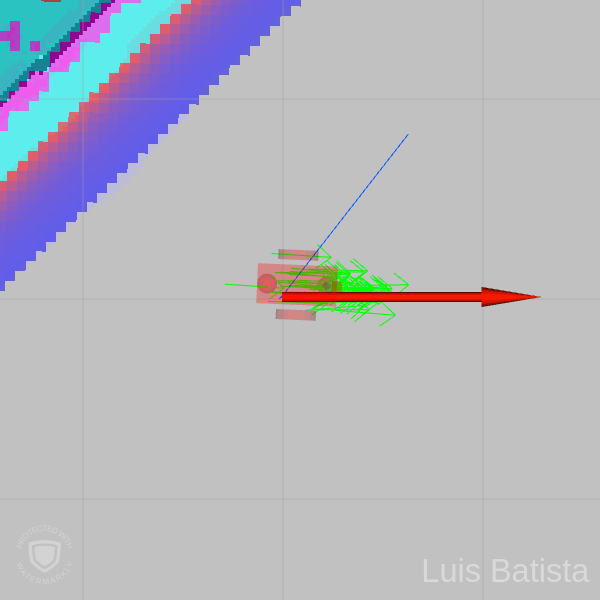
\includegraphics[width=.95\linewidth]{ub_final.png}
  \caption{Udacity Bot}
  \label{fig:ub-final}
\end{subfigure}%
\begin{subfigure}{.5\linewidth}
  \centering
  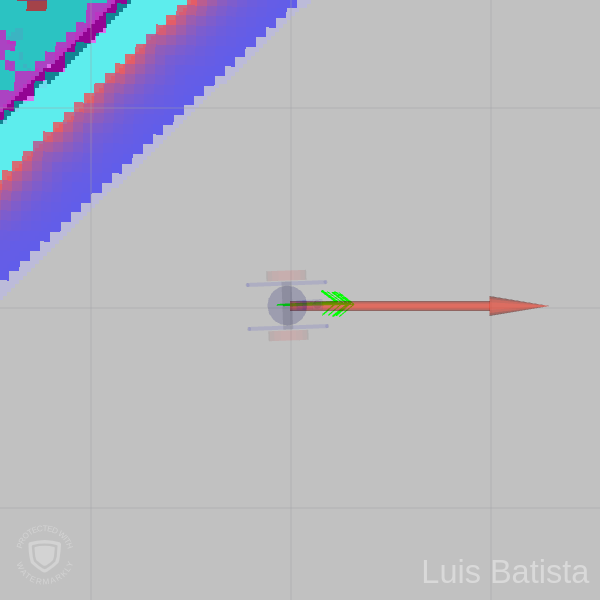
\includegraphics[width=.95\linewidth]{r2d2_final.png}
  \caption{R2D2 Bot}
  \label{fig:r2d2-final}
\end{subfigure}
\caption{Robots in Final Position}
\label{fig:final}
\end{figure}


Figure \ref{fig:initial-position} shows the initial distribution of the particles. In the case of the R2D2 robot, the higher number of particles incurs in a higher probability that some particles are correctly placed close to the actual location of the robot.


\begin{figure}[H]
\centering
\begin{subfigure}{.5\linewidth}
  \centering
  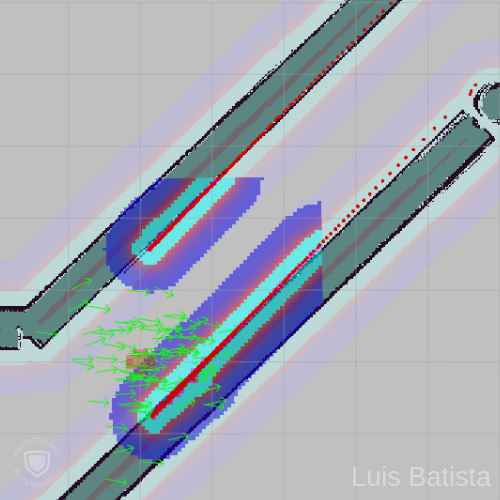
\includegraphics[width=.95\linewidth]{ub_1.png}
  \caption{Udacity Bot}
  \label{fig:ub-1}
\end{subfigure}%
\begin{subfigure}{.5\linewidth}
  \centering
  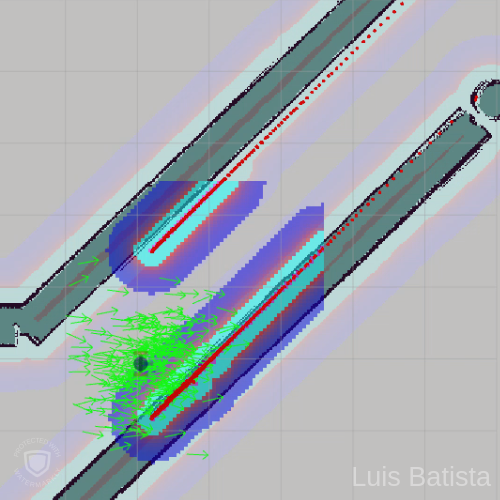
\includegraphics[width=.95\linewidth]{r2d2_1.png}
  \caption{R2D2 Bot}
  \label{fig:r2d2-1}
\end{subfigure}
\caption{Initial Position}
\label{fig:initial-position}
\end{figure}

As a result, the particles tend to converge quickly after the R2D2 starts moving. The Figure \ref{fig:r2d2-2} shows clearly shows the difference in the distribution of the particles after each robot has moved almost the same distance. 

\begin{figure}[H]
\centering
\begin{subfigure}{.5\linewidth}
  \centering
  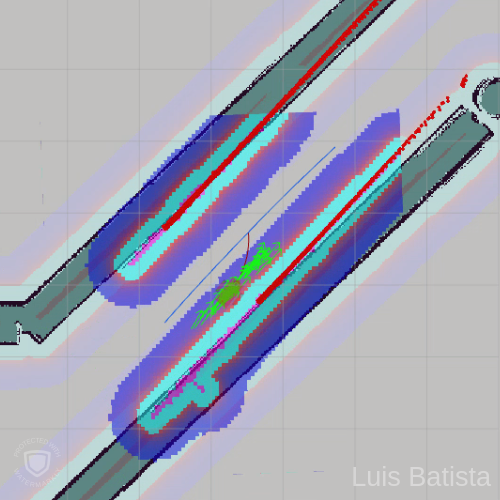
\includegraphics[width=.95\linewidth]{ub_2.png}
  \caption{Udacity Bot}
  \label{fig:ub-2}
\end{subfigure}%
\begin{subfigure}{.5\linewidth}
  \centering
  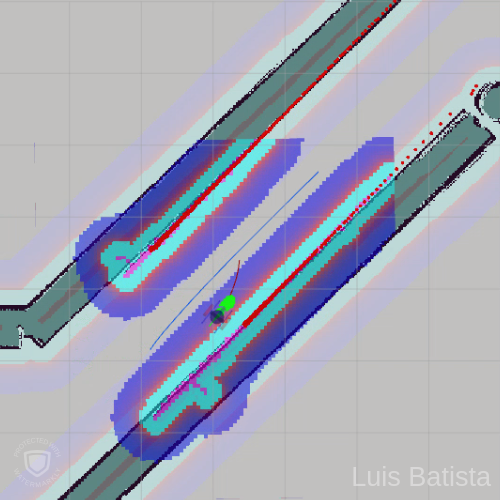
\includegraphics[width=.95\linewidth]{r2d2_2.png}
  \caption{R2D2 Bot}
  \label{fig:r2d2-2}
\end{subfigure}
\caption{First Particle Convergence}
\label{fig:conv1}
\end{figure}

In the case of the Udacity Bot, the particles start to converge only when it is close to making the first sharp turn to the right at the end of the middle passage (Figure \ref{fig:ub-3}). Despite the longer time to converge, the robot is able to follow a smooth path from the start to the goal position.

\begin{figure}[H]
\centering
\begin{subfigure}{.5\linewidth}
  \centering
  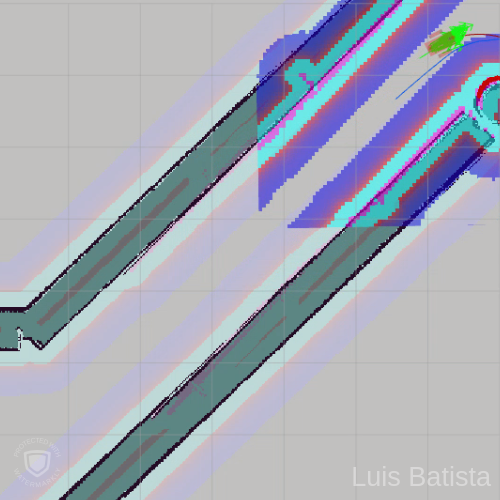
\includegraphics[width=.95\linewidth]{ub_3.png}
  \caption{Udacity Bot}
  \label{fig:ub-3}
\end{subfigure}%
\begin{subfigure}{.5\linewidth}
  \centering
  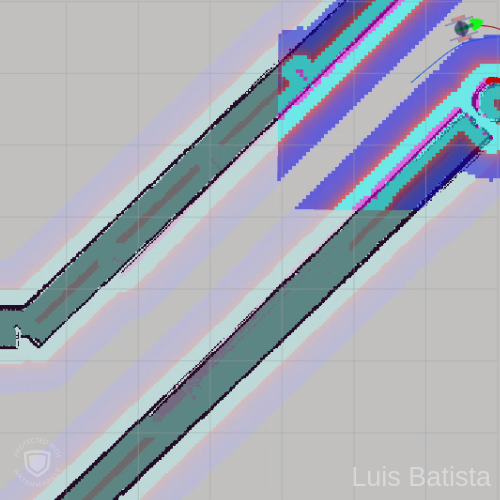
\includegraphics[width=.95\linewidth]{r2d2_3.png}
  \caption{R2D2 Bot}
  \label{fig:r2d2-3}
\end{subfigure}
\caption{First Particle Convergence}
\label{fig:conv2}
\end{figure}

The R2D2 Bot have achieved better performance using the parameters described on Tables \ref{tab:amcl-param} and \ref{tab:blc-param}. Nevertheless, as described previously in Section \ref{sec-modeldesign}, the physical characteristics and the sensor placement is very similar on both robots. It allows to use the better-tunned paraments also in the Udacity Bot and get very similar results. The Figure \ref{fig:ub-final2} shows the benchmark robot reaching the final position with converged particles by using the same parameters as the R2D2 Bot.

\begin{figure}[H]
\centering
  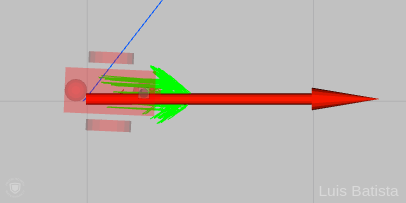
\includegraphics[width=0.6\linewidth]{ub_final2.png}
  \caption{Udacity Bot with tunned AMC Parameters}
  \label{fig:ub-final2}
\end{figure}


\section{Discussion}


The results clearly indicate that increasing the number of particles and updating the particles in shorter cycles, resulted in a better convergence. This explains why parameters used for the R2D2 Bot performed better when comparing to the parameters used for the Udacity Bot.

It was also noticed that the distribution of the particles becomes less precise when the robot reaches the final position. As the orientation is facing towards an open area, the distance of the objects in larger, increasing the noise and reducing the accuracy of the estimated pose.

The AMCL algorithm is a feasible option to be used in cases where global localization is necessary. If the initial position of the robot was unknown, the particles would have to be evenly distributed across the entire map. The required computational resources would decrease as the particles converged to the actual position of the robot. However, the algorithm would not be sufficient in case of the kidnapped robot problem. Robustness for such situations become mandatory in real-world robots such as autonomous vacuum cleaner for example.

While this report focused mostly on the evaluation of the AMCL algorithm for localization, there are some situations where the EKF would be a better option. This would be the case if the available hardware resources are very limited and the primary goal is to solve local localization.


\section{Conclusion / Future work}
This project successfully achieved the goal of learning how to use and adjust the parameters for localization using AMCL algorithm. Using the simulated environment, it was possible the explore the localization parameters and quickly observe the results. It was also possible to experiment with the computational impact when trying to optimize the results.  

\subsection{Modifications for Improvement}

Despite reaching the initial goals there are several improvements and further investigation that can be done.

\begin{itemize}
\item Adjust amlc parameters according to the expected noise from the sensors.
\item Modify the move\_base parameters to get better path planning results.
\item Make use of additional sensors in different locations of the robot.
\item Explore the impact of physical characteristics of the robot, such as mass, inertia, and friction coefficients. 
\item Repeat the tests using a more realist robot model, such as the TurtleBot 3 available in ROS.
\end{itemize}

\subsection{Hardware Deployment}
Exploring the results on simulation is great for learning and also important for initial adjustments. In order to deploy in real hardware, it is very important to readjust the parameters according to the hardware performance. In case of using limited hardware, such as a Raspberry PI, the AMCL could be processed in a more powerful computer.
The following steps provide an outline of the required tasks.
\begin{enumerate}
\item Recreate simulation model based on a real robot.
\item Adjust the AMCL and Move Base parameters according to the new robot.
\item Deploy and adjust the frequency of update according to computation resources available.
\item Test and tune the parameters.
\end{enumerate}

\bibliography{bib}
\bibliographystyle{ieeetr}

\end{document}
